% Header
\documentclass[a4paper]{article}%      autres choix : book, report
\usepackage[utf8]{inputenc}%           gestion des accents (source)
\usepackage[T1]{fontenc}%              gestion des accents (PDF)
\usepackage[francais]{babel}%          gestion du français
\usepackage{textcomp}%                 caractères additionnels
\usepackage{mathtools,amssymb,amsthm}% packages de l'AMS + mathtools
\usepackage{lmodern}%                  police de caractère
\usepackage[top=2cm,left=2cm,right=2cm,bottom=2cm]{geometry}%     gestion des marges
\usepackage{graphicx}%                 gestion des images
\usepackage{array}%                    gestion améliorée des tableaux
\usepackage{calc}%                     syntaxe naturelle pour les calculs
\usepackage{titlesec}%                 pour les sections
\usepackage{titletoc}%                 pour la table des matières
\usepackage{fancyhdr}%                 pour les en-têtes
\usepackage{titling}%                  pour le titre
\usepackage{enumitem}%                 pour les listes numérotées
\usepackage{hyperref}%                 gestion des hyperliens

\hypersetup{pdfstartview=XYZ}%         zoom par défaut

\setlength{\droptitle}{-5em}   % This is your set screw
\title{\vspace{1.5cm}Graph Mining Project}
\author{Mickaël LAURENT}
\date{\vspace{-5ex}}

\pagenumbering{gobble}
\DeclarePairedDelimiter\ceil{\lceil}{\rceil}
\DeclarePairedDelimiter\floor{\lfloor}{\rfloor}

\begin{document}

	\maketitle

	\section{Implementation}

	I have implemented this project in Python 3.
	The implementation of the two algorithms are in the file \textit{clustering.py}.

	\paragraph{Offline algorithm} The offline algorithm is implemented in the function \textit{robust\_clustering}.
	It calls the function \textit{robust\_clustering\_with\_radius} with the best \textit{optimal radius} argument by performing a dichotomic search.
	The function \textit{robust\_clustering\_with\_radius} has a parameter \textit{unrestricted\_centers}, which can be set True if we want to use
	the slightly modified version of this algorithm used by the streaming algorithm.\\

	\begin{tabular}{|l|l|l|}
		\hline
		\textit{Unrestricted\_center} & Centers & Guarantee \\
		\hline
		False & Among input points & 3-approximation \\
		True & Unrestricted & 4-approximation \\
		\hline
	 \end{tabular}\\

	\paragraph{Streaming algorithm} The streaming algorithm is implemented in the class \textit{StreamingClustering}.
	I used a class so that we can initialize and use multiple independant instances
	of the streaming clustering algorithm in the same time.\\

	I have also implemented the parallelized version of this algorithm in order to have better guarantees.
	It is implemented in the class \textit{ParallelStreamingClustering} that takes the parameter \textit{m} as input.
	Indeed, it is not really a parallel implementation: it is just a sequential execution of multiple instances
	of \textit{StreamingClustering}. As a consequence, using this implementation with $m=2$ will probably
	take twice more time than using it with $m=1$.

	\paragraph{Testing} In order to test my implementation, I have designed an interactive tool that uses
	\textit{matplotlib}. You can test it by running the file \textit{test\_interactive.py}. It allows the user to
	add some points by clicking on the canvas, to see the output of the streaming algorithm in live and to compare it
	with the offline algorithm.

	\section{Upper-bound of an optimal solution}

	\paragraph{Method}
	In order to find an upper bound, I have made a geometric reasoning.
	We use an euclidean distance, and the coordinates of the dataset go from -180 to 180 on the x-axis, and -90 to 90 on the y-axis.
	So we can represent the space of the dataset by a rectangle of dimensions 360x180.\\

	As we want at most $k=20$ clusters, we should find out what is the minimal radius $r$ such that 20 circles of radius $r$
	can cover the entire 360x180 rectangle. I have solved this problem approximately by noticing that 18 squares of dimension 60x60
	can cover a 360x180 rectangle, and so can do 18 circles of radius $\frac{60}{2}\sqrt{2}$ (of course, they will overlap, so it may not be optimal).
	It gives us the following upper bound for the optimal solution: 42.

	\paragraph{Limits}

	This upper-bound is very approximative. Indeed, it assumes the points to be distributed over the whole 360x180 rectangle:
	if all the points were distributed into a few small areas with nothing around, it would be possible to cover all the points without covering
	the whole surface of the rectangle. In order to observe that, I have drawn all the point on a 360x180 canvas using \textit{matplotlib} (see image below).
	Altough we can see some almost-empty areas, it does not seem to be possible to cover all the points without covering almost the entire rectangle,
	so our upper-bound may not be \textbf{so} bad.\\

	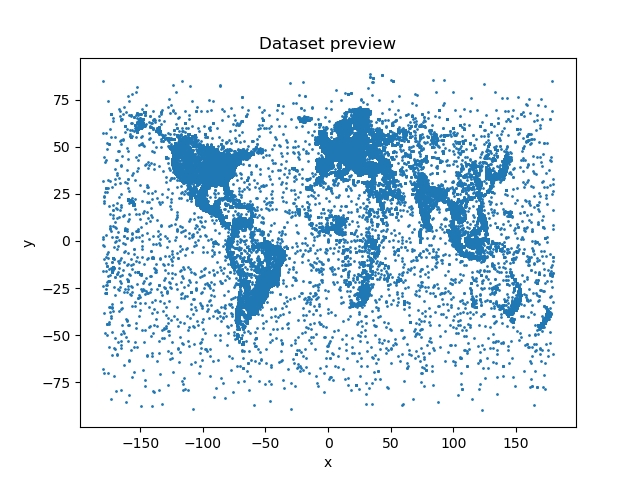
\includegraphics{dataset_preview}

	Another thing to notice is that our invariant does not take $z$ (the number of outliers) into account.
	Indeed, I have not found any idea to take it into account without performing a way more detailled analysis.\\

	Knowing all of that, it is probably not the best upper-bound.
	However, we should keep in mind that 42 is also the \textit{Answer to the Ultimate Question of Life, the Universe, and Everything}.
	Moreover, I am personally convinced that \textit{the Ultimate Question of Life, the Universe, and Everything} is the following:\\
	\textit{What is the minimal radius $r$ such that we can cover all the points described in the well-known dataset twitter\_1000000.txt with
	20 circles of radius $r$, using an eucliden distance and allowing to ignore at most 10 of these points ?},\\
	in wich case our upper-bound would be optimal.
	Consequently, I have decided to keep this upper-bound.

	\section{Plots and discussion}

	I have realized the plots suggested in the subject not only for $m=1$, but also for $m=3$ and $m=5$ because the
	results I obtained for $m=1$ seemed quite weird to me. Comparing them to the results obtained with $m=3$ and $m=5$
	allowed me to propose an explanation.\\

	First of all, let's remind the guarantees of the streaming algorithm:
	\begin{enumerate}
		\item Approximation factor: $4+\epsilon$ with $\epsilon=(\eta/\alpha)\alpha^{1/m}=4\times4^{1/m}$
		\item Memory used: $\mathcal{O}(\epsilon^{-1}kz)$
		\item Running time: $\mathcal{O}(\epsilon^{-1}(kzn + (kz)^2\log P))$ with $P$ fixed for a given instance\\
		(\textit{$P$ is the ratio of the optimal radius to the shortest distance between any two distinct input points})
	\end{enumerate}

	In our setting, $kzn >> (kz)^2\log P$ so running time can be approximated by $\mathcal{O}(\epsilon^{-1}(kzn))$.

	It gives the following expectations:\\

	\begin{tabular}{|l|l|l|l|}
		\hline
		With fixed $z$ & $m=1$ & $m=3$ & $m=5$ \\
		\hline
		Approximation factor & 16 & 6.3 & 5.3 \\
		Memory used & $M$ & $2.5M$ & $3M$ \\
		Running time & $T$ & $2.5T$ & $3T$ \\
		\hline
	 \end{tabular}\\

	\begin{tabular}{|l|l|l|l|l|l|}
		\hline
		With fixed $m$ & $z=10$ & $z=20$ & $z=30$ & $z=40$ & $z=50$ \\
		\hline
		Memory used & $M$ & $2M$ & $3M$ & $4M$ & $5M$ \\
		Running time & $T$ & $2T$ & $3T$ & $4T$ & $5T$ \\
		\hline
	 \end{tabular}\\

	Below are the plots I have obtained. Blue, orange and green curves are respectively with $m=1$, $m=3$ and $m=5$.
	Note that the approximation factor is computed using the upper-bound found in the previous section, which does not
	take the parameter $z$ into account. Consequently, when refering to the \textit{approximation factor},
	it actually refers to the ratio of the radius found by the algorithm for a given value of z to the approximate
	optimal radius for z=0.

	\begin{figure}[h]
		\caption{Approximation factor depending on $z$}
		\centering
		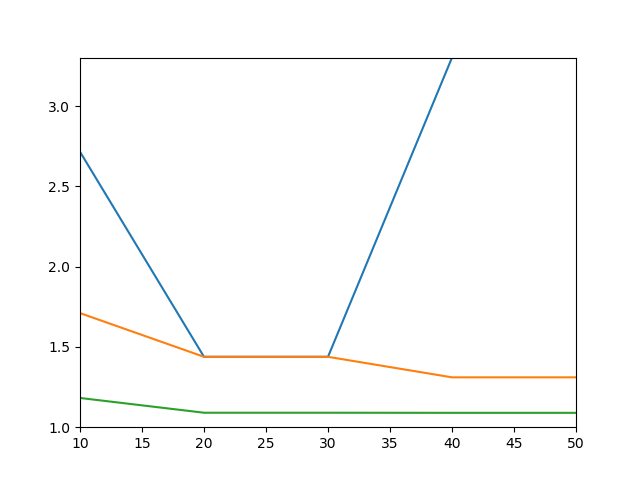
\includegraphics[width=0.55\textwidth]{curve_r}
	\end{figure}
	\begin{figure}[h]
		\caption{Running time depending on $z$}
		\centering
		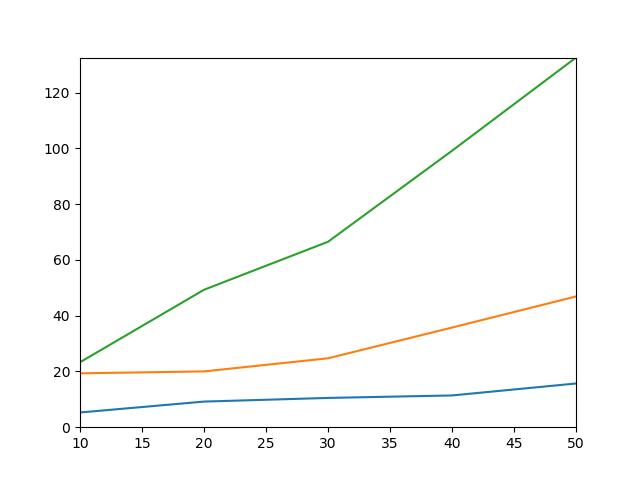
\includegraphics[width=0.55\textwidth]{curve_t}
	\end{figure}

	Concerning the approximation factor, the guarantee is respected for each curve.
	However, for the blue curve ($m=1$), the evolution of the radius found when $z$ increase is quite surprising:
	indeed, a solution found for $z=10$ is still valid for $z=50$, so we could expect the algorithm to
	find a solution at least as good when $z=50$ as when $z=10$. There does not seem to be this problem when $m=3$ and $m=5$.\\
	
	Here is a possible explanation. I think that the result of this algorithm is very dependent on the initial radius
	computed during the initialization phase. The duration of this phase depends on $z$, and so choosing a different
	$z$ can change the value of the initial radius in a quite random way (this can explain the behavior observed
	with the blue curve). However, when increasing $m$, we run more instances of this algorithm with each time
	a different value for the initial radius (and only the best result is returned). This tends to reduce this
	\textit{random factor} observed when $m=1$. For the same reason, it also improves the results in a significant way:
	for $z=50$, the approximation factor with $m=5$ is more than 3 times better than with $m=1$.\\

	Concerning the running time, it seems to increase slower than expected for $m=1$ (good news!).
	It is not the case for $m=5$, for which the running time for $z=50$ is more than 3 times greater than the running time for $z=10$.
	However, my implementation of the parallelized version is not efficient (it is actually sequential) so we should not
	compare these measures with the bounds given in the paper.

	

\end{document}